\documentclass[11pt,a4paper]{report}

% ================== PACKAGES ==================
\usepackage[a4paper,margin=1in]{geometry}
\usepackage{setspace}
\usepackage{graphicx}
\usepackage{fancyhdr}
\usepackage{titlesec}
\usepackage{multicol}
\usepackage{hyperref}
\usepackage{tikz}
\usepackage{xcolor}
\usepackage{array}
\usepackage{caption}
\usepackage{subcaption}
\usepackage{booktabs}
\usepackage{amsmath,amssymb}
\usepackage{multirow}
\usepackage{float}
\usepackage{lmodern}
\usepackage{times}
\usepackage{parskip}
\usepackage{rotating}
\usepackage{pdflscape}
\usepackage{natbib}
\usepackage{siunitx}
\usepackage{pgfplots}
\usepackage{microtype}
\pgfplotsset{compat=1.18}

\usetikzlibrary{shapes.geometric, arrows.meta, positioning, calc, fit}
\usepackage{everypage-1x}

\graphicspath{{./}}

% ================== SPACING ==================
\setstretch{1.3}
\setlength{\columnsep}{0.7cm}
\setlength{\emergencystretch}{3em}
\tolerance=2000
\captionsetup{font=small, labelfont=bf}

% ================== FLOAT PLACEMENT ==================
\renewcommand{\topfraction}{0.9}
\renewcommand{\bottomfraction}{0.8}
\renewcommand{\textfraction}{0.1}
\renewcommand{\floatpagefraction}{0.85}
\renewcommand{\dbltopfraction}{0.9}
\renewcommand{\dblfloatpagefraction}{0.85}
\setcounter{topnumber}{3}
\setcounter{dbltopnumber}{3}
\setcounter{totalnumber}{5}

% ================== BORDER BOX FOR EACH PAGE ==================
\newif\ifblankpage
\AddEverypageHook{%
  \ifblankpage\else
  \begin{tikzpicture}[remember picture,overlay]
    \draw[line width=1pt]
      ($(current page.north west)+(1cm,-1cm)$)
      rectangle
      ($(current page.south east)+(-1cm,1cm)$);
  \end{tikzpicture}%
  \fi
}
% Empty back page for single-sided printing: no border, header or page number, not counted.
\newcommand{\blankpage}{%
  \clearpage\blankpagetrue\thispagestyle{empty}\null\clearpage
  \blankpagefalse\addtocounter{page}{-1}}

% ================== HEADER & FOOTER ==================
\pagestyle{fancy}
\fancyhf{}
\fancyhead[L]{RGUKT Nuzvid}
\fancyhead[R]{Phase 3 Project Report}
\fancyfoot[R]{Page \thepage}
\renewcommand{\headrulewidth}{0pt}
\fancypagestyle{plain}{\fancyhf{}\fancyhead[L]{RGUKT Nuzvid}\fancyhead[R]{Phase 3 Project Report}\fancyfoot[R]{Page \thepage}}

% ================== TITLE FORMAT ==================
% Chapters run on in the same page instead of always starting a new page.
\titleclass{\chapter}{straight}
\titleformat{\chapter}{\bfseries\Large}{\thechapter.}{0.6em}{}
\titleformat{\section}{\bfseries\large}{\thesection.}{0.6em}{}
\titleformat{\subsection}{\bfseries\normalsize}{\thesubsection.}{0.6em}{}
\titlespacing*{\chapter}{0pt}{14pt}{6pt}
\titlespacing*{\section}{0pt}{9pt}{3pt}
\titlespacing*{\subsection}{0pt}{6pt}{2pt}
\renewcommand{\bibname}{References}

% ================== HYPERREF SETUP ==================
\hypersetup{colorlinks=true, linkcolor=blue, citecolor=blue, urlcolor=blue}

% =======================================================
\begin{document}

% =======================================================
% ================== TITLE PAGE =========================
% =======================================================
\begin{center}
\onehalfspacing

\textbf{\LARGE Domain Sensitivity-Guided Selective Adaptation\\[0.3cm]
for Remote Sensing Segmentation} \\[0.4cm]
\textit{Phase 3: Budget-Matched LoRA Placement in Prithvi-EO-2.0} \\[1cm]

\textit{A Phase 3 Project Report}\\[0.2cm]
Submitted in partial fulfillment for the award of the degree of \\[0.4cm]

\textbf{BACHELOR OF TECHNOLOGY}\\[0.2cm]
\textbf{in} \\[0.2cm]
\textbf{COMPUTER SCIENCE AND ENGINEERING}\\[1cm]

Submitted by \\[0.3cm]
\textbf{A. Siva Teja Reddy (N211077)} \\
\textbf{A. Sree Harsh (N210264)} \\
\textbf{B. Likhith (N210781)} \\
\textbf{P. Janaki Ram (N210686)} \\
\textbf{A. Srinivas Reddy (N210054)} \\[1cm]

\textit{Under the Esteemed Guidance of} \\[0.3cm]
\textbf{Dr.~Nagarjuna Devi}\\
Department of CSE, RGUKT Nuzvid \\[1cm]


\includegraphics[width=4cm]{rgukt_logo.png}\\[0.8cm]

\textbf{DEPARTMENT OF COMPUTER SCIENCE AND ENGINEERING}\\
\textbf{RAJIV GANDHI UNIVERSITY OF KNOWLEDGE TECHNOLOGIES, NUZVID}\\
Nuzvid, Eluru, Andhra Pradesh, 521202. \\[0.4cm]

\textit{2026 to 2027}
\end{center}

\blankpage

% =======================================================
% ============ CERTIFICATE OF COMPLETION ================
% =======================================================
\begin{center}
\onehalfspacing

\includegraphics[width=4cm]{rgukt_logo.png}\\[0.5cm]
\textbf{\Large DEPARTMENT OF COMPUTER SCIENCE AND ENGINEERING}\\[0.2cm]
\textbf{Rajiv Gandhi University of Knowledge Technologies, Nuzvid}\\
Nuzvid, Eluru, Andhra Pradesh, 521202.\\[0.8cm]
\textbf{\underline{CERTIFICATE OF COMPLETION}}\\[0.8cm]
\end{center}

This is to certify that the Phase 3 project report entitled \textbf{``Domain Sensitivity-Guided Selective Adaptation for Remote Sensing Segmentation''} is the bonafide work of \textbf{A. Siva Teja Reddy (N211077), A. Sree Harsh (N210264), B. Likhith (N210781), P. Janaki Ram (N210686)} and \textbf{A. Srinivas Reddy (N210054)}, carried out under the supervision of \textbf{Dr.~Nagarjuna Devi}, Department of CSE, RGUKT Nuzvid.\\[0.3cm]

This report covers the third phase of the major project, done during the academic session \textbf{2026 to 2027}. The work tests, under a protocol fixed in advance, whether choosing which layers of a large geospatial model to fine-tune is better than spreading the same small parameter budget over every layer.\\[0.5cm]

\vspace{1cm}
\noindent
\begin{multicols}{2}
\begin{flushleft}
\rule{6cm}{0.4pt} \\[-0.2cm]
\textbf{Dr.~Nagarjuna Devi} \\
Project Guide,\\
Department of CSE,\\
RGUKT Nuzvid.
\end{flushleft}

\columnbreak

\begin{flushright}
\rule{6cm}{0.4pt} \\[-0.2cm]
\textbf{Head of the Department}\\
Department of CSE,\\
RGUKT Nuzvid.
\end{flushright}
\end{multicols}

\blankpage

% =======================================================
% ============ CERTIFICATE OF EXAMINATION ===============
% =======================================================
\begin{center}

\includegraphics[width=4cm]{rgukt_logo.png}\\[0.5cm]
\textbf{\Large DEPARTMENT OF COMPUTER SCIENCE AND ENGINEERING}\\[0.2cm]
\textbf{Rajiv Gandhi University of Knowledge Technologies, Nuzvid}\\
Nuzvid, Eluru, Andhra Pradesh, 521202.\\[0.8cm]
\textbf{\underline{CERTIFICATE OF EXAMINATION}}\\[0.8cm]
\end{center}

This is to certify that the Phase 3 project report entitled \textbf{``Domain Sensitivity-Guided Selective Adaptation for Remote Sensing Segmentation: Budget-Matched LoRA Placement in Prithvi-EO-2.0''}, submitted by \textbf{A. Siva Teja Reddy (N211077), A. Sree Harsh (N210264), B. Likhith (N210781), P. Janaki Ram (N210686)} and \textbf{A. Srinivas Reddy (N210054)}, has been examined and approved as a study carried out and presented in a manner required for its acceptance in the final year of \textbf{Bachelor of Technology} in Computer Science and Engineering.\\[0.3cm]

This approval does not necessarily endorse or accept every statement made or opinion expressed but signifies the acceptance of the report for the purpose for which it has been submitted.\\[0.5cm]

\vspace{1cm}
\noindent
\begin{multicols}{2}
\begin{flushleft}
\rule{6cm}{0.4pt} \\[-0.2cm]
\textbf{Dr.~Nagarjuna Devi}\\
Project Guide, Department of CSE,\\
RGUKT Nuzvid.
\end{flushleft}

\columnbreak

\begin{flushright}
\rule{6cm}{0.4pt} \\[-0.2cm]
\textbf{Project Examiner}\\
Department of CSE,\\
RGUKT Nuzvid.
\end{flushright}
\end{multicols}

\blankpage

% =======================================================
% ================== DECLARATION PAGE ===================
% =======================================================
\begin{center}

\includegraphics[width=4cm]{rgukt_logo.png}\\[0.5cm]
\textbf{\Large DEPARTMENT OF COMPUTER SCIENCE AND ENGINEERING}\\[0.2cm]
\textbf{Rajiv Gandhi University of Knowledge Technologies, Nuzvid}\\
Nuzvid, Eluru, Andhra Pradesh, 521202.\\[0.8cm]
\textbf{\underline{DECLARATION}}\\[0.8cm]
\end{center}

We, \textbf{A. Siva Teja Reddy (N211077), A. Sree Harsh (N210264), B. Likhith (N210781), P. Janaki Ram (N210686)} and \textbf{A. Srinivas Reddy (N210054)}, hereby declare that the Phase 3 project report entitled \textbf{``Domain Sensitivity-Guided Selective Adaptation for Remote Sensing Segmentation''}, completed under the guidance of \textbf{Dr.~Nagarjuna Devi}, Department of CSE, RGUKT Nuzvid, is a record of our own work carried out during the academic session \textbf{2026 to 2027}.\\[0.4cm]

We also declare that this work has not been submitted to any other university or institution for the award of any degree or diploma, and that all sources used have been properly cited.

\vspace{0.8cm}
\noindent
\textbf{Date:} \today\\[0.3cm]
\textbf{Place:} Nuzvid

\vspace{0.6cm}
\begin{flushright}
\textbf{A. Siva Teja Reddy}\\
\textbf{A. Sree Harsh}\\
\textbf{B. Likhith}\\
\textbf{P. Janaki Ram}\\
\textbf{A. Srinivas Reddy}
\end{flushright}

\blankpage

% =======================================================
% ================= ACKNOWLEDGEMENT =====================
% =======================================================
\begin{center}
\textbf{\Large ACKNOWLEDGEMENT}
\end{center}

\vspace{0.5cm}
We would like to thank our guide \textbf{Dr.~Nagarjuna Devi}, Department of Computer Science and Engineering, RGUKT Nuzvid, for the guidance and encouragement we received throughout this project. The regular reviews and suggestions helped us a lot in deciding what to test and how to report it.

We are grateful to the \textbf{Head of the Department of CSE}, RGUKT Nuzvid, for providing the facilities and the academic environment needed for this work.

We also thank all the faculty members of the Department of Computer Science and Engineering. What we learned in their courses over the last few years is the base on which this project is built.

We thank the International Society for Photogrammetry and Remote Sensing (ISPRS) for giving us access to the Potsdam and Vaihingen datasets, and the IBM and NASA teams for releasing the Prithvi-EO-2.0 model weights publicly. We also used PyTorch and timm, and we thank the people who maintain them.

Finally, we thank our families for their support and our batchmates at RGUKT Nuzvid for their encouragement.

\vspace{1.5cm}
\begin{flushright}
\textbf{A. Siva Teja Reddy}\\
\textbf{A. Sree Harsh}\\
\textbf{B. Likhith}\\
\textbf{P. Janaki Ram}\\
\textbf{A. Srinivas Reddy}
\end{flushright}

\blankpage

% =======================================================
% =================== ABSTRACT PAGE =====================
% =======================================================
\begin{center}
\textbf{\Large ABSTRACT}
\end{center}

\vspace{0.5cm}
Geospatial foundation models such as Prithvi-EO-2.0 lose accuracy when moved to images from a new city or sensor, and Low-Rank Adaptation (LoRA) is a cheap way to adapt them. In Phase 2 of this project (Potsdam to Vaihingen) we found that our label-free Domain Sensitivity Score (DSS) mostly ranked blocks by depth and did not pick useful blocks better than chance, while LoRA in the middle blocks helped most. Phase 3 tests these findings properly and asks the efficiency question that Phase 2 left open: at a fixed parameter budget, is it better to put LoRA in a few chosen blocks or to spread it thinly over all blocks?

We reversed the transfer direction (ISPRS Vaihingen to ISPRS Potsdam), so the Potsdam labels were new to us, and froze every step of the protocol before running it. Stage A froze the Potsdam split (20 training, 8 validation and 10 test tiles). Stage B computed and hashed six block scores: four label-free signals (DSS-R2, GSD-perturbation sensitivity, input-output similarity and activation norm) and two label-using references (Fisher and LogME). Stage C trained LoRA in each of the 24 blocks with three seeds (75 runs). Every block helped (+0.021 to +0.052 mIoU), but no label-free signal passed our screening gate, so the protocol selected one confirmatory test: is a frozen depth prior (blocks L13 to L15, rank 8) non-inferior to uniform rank-1 LoRA on all 24 blocks, which uses exactly the same 98,304 LoRA parameters? Stage D trained 10 arms (67 new runs), and all 70 final models were then scored once on the 10 locked Potsdam test tiles.

The confirmatory test failed clearly. On the test set, the prior's 3 blocks scored 0.0341 mIoU below uniform rank 1 (95\% interval $-0.0392$ to $-0.0291$, margin $-0.010$) and were worse on all 10 seeds. Uniform rank 1 reached 0.615 test mIoU, a gain of +0.087 over the decoder-only baseline (0.529). That is 88\% of the gain of standard rank-8 LoRA on all blocks (+0.099) with one eighth of its LoRA parameters. Every 3-block arm gained only +0.042 to +0.062, and no score-chosen set beat randomly chosen blocks. The arm ranking was identical on validation and test. Our conclusion is a clear, pre-registered negative result for block selection and a positive one for budget spreading: at a fixed LoRA budget, spreading a small rank over every block beats concentrating it in a few selected blocks.

\textbf{Keywords:} domain shift, remote sensing, semantic segmentation, Prithvi-EO-2.0, LoRA, parameter-efficient fine-tuning, layer selection, pre-registration, ISPRS Potsdam, ISPRS Vaihingen.

\blankpage

\pagenumbering{roman}
\tableofcontents
\newpage
\listoffigures
\listoftables
\blankpage

\pagenumbering{arabic}
\twocolumn
\setstretch{1.12}

% =======================================================
% ============ CHAPTER 1: INTRODUCTION ==================
% =======================================================
\chapter{Introduction}

\section{Background}

Large geospatial foundation models such as Prithvi \cite{jakubik2023foundation,szwarcman2024prithvi} are pretrained on huge archives of Earth observation data and then adapted to new tasks with a small labelled dataset. When the new images come from a different city, camera or ground resolution, the model has to deal with domain shift \cite{bendavid2010theory,tuia2016domain}. Full fine-tuning of the 300 million parameter Prithvi-EO-2.0 model is expensive, so parameter-efficient methods such as LoRA \cite{hu2022lora} are used instead. LoRA is normally added to every transformer block with the same rank. Earlier work suggests that adapting only some layers can be just as good \cite{lee2023surgical}, which raises the question of which layers to choose.

\section{What Phase 2 Found}

Our project, DSSA (Domain Sensitivity-Guided Selective Adaptation), proposed choosing blocks with a Domain Sensitivity Score (DSS) computed from unlabelled images. Phase 2 tested this on transfer from ISPRS Potsdam to ISPRS Vaihingen with 75 single-block runs. The results were:

\begin{enumerate}
    \item Which block is adapted matters. One adapted block raised the validation mIoU from 0.518 (decoder only) to as much as 0.555 (block L16).
    \item The gain was largest in the middle blocks (L11 to L17). This pattern was found after looking at the results.
    \item The DSS ranking was almost a depth ranking (Spearman 0.94). Once depth was removed, its correlation with the gain was only 0.076, and its top-$k$ picks were no better than random picks.
\end{enumerate}

Phase 2 also left an important gap. We never compared selective LoRA with LoRA in all blocks, so the efficiency part of our original hypothesis was untested.

\section{Phase 3 Research Questions}

Phase 3 was designed to answer three questions, with the full protocol written down and frozen before each stage:

\begin{enumerate}
    \item \textbf{Replication.} Does the single-block utility pattern hold in the reverse direction (Vaihingen to Potsdam), where the target labels have never been used?
    \item \textbf{Selection signals.} Can any block score, label-free or label-using, pick useful blocks better than a fixed depth prior or a random choice?
    \item \textbf{Select or spread.} At exactly the same number of LoRA parameters, is adapting 3 chosen blocks at rank 8 as good as adapting all 24 blocks at rank 1?
\end{enumerate}

\section{Contributions}

\begin{enumerate}
    \item A pre-registered protocol (versions 1 to 4, a red-team review and a decision register) that fixed the split, the scores, the thresholds, the arms, the seeds and the analysis before each stage was run.
    \item A full single-block utility map on Potsdam (75 runs) and a screening test of six block scores against it.
    \item A budget-matched comparison of 10 adaptation arms (67 new runs plus 3 reused baselines), with 10 seeds for the main arms.
    \item A single, frozen opening of the Potsdam test set for all 70 models, with one confirmatory contrast.
    \item A clear result: spreading LoRA thinly over every block beats concentrating it in a few chosen blocks, and no block score we tried beats random selection.
\end{enumerate}

\section{Organization of the Report}

Chapter~\ref{ch:related} adds the related work needed for Phase 3. Chapter~\ref{ch:method} describes the block scores, the screening gate, the Stage D arms and the confirmatory test. Chapter~\ref{ch:setup} gives the data split, the training settings and the safeguards. Chapter~\ref{ch:results} reports Stages A to D and the test results. Chapter~\ref{ch:discussion} discusses the results and their limits, and Chapter~\ref{ch:conclusion} concludes.

% =======================================================
% ============ CHAPTER 2: RELATED WORK ==================
% =======================================================
\chapter{Related Work}
\label{ch:related}

\section{Recap from Phase 2}

The Phase 2 report reviewed domain adaptation in remote sensing \cite{tuia2016domain,ganin2016domain}, geospatial foundation models \cite{he2022masked,cong2022satmae,jakubik2023foundation,szwarcman2024prithvi}, parameter-efficient fine-tuning \cite{houlsby2019parameter,hu2022lora,zhang2023adalora,lee2023surgical} and methods for comparing representations across layers \cite{raghu2017svcca,kornblith2019similarity,gretton2012kernel}. We do not repeat that review here and only add the work that the new Phase 3 scores are based on.

\section{Label-Using Block Scores}

Two of our Phase 3 scores use target training labels. Fisher information measures how strongly the training loss reacts to a change in a parameter, and it is widely used to estimate parameter importance, for example in elastic weight consolidation \cite{kirkpatrick2017overcoming}. We use the squared gradient of the loss with respect to each block's LoRA weights as a Fisher-style importance score. LogME \cite{you2021logme} estimates how well a frozen feature set can predict labels by computing the evidence of a Bayesian linear model, and it was proposed to rank pretrained models for transfer. We apply it per block to the frozen patch tokens. Because both scores use labels, we treat them as references and not as label-free candidates.

\section{Uniform Low-Rank Budgets}

Plain LoRA spreads one rank over all chosen weight matrices, and AdaLoRA \cite{zhang2023adalora} moves rank between layers during training. A simple question that is rarely tested directly is whether a fixed number of LoRA parameters is better spent as a high rank in a few layers or a very low rank in every layer. Our Stage D answers this for Prithvi-EO-2.0 by comparing 3 blocks at rank 8 with 24 blocks at rank 1, which have exactly the same number of LoRA parameters.

% =======================================================
% ============ CHAPTER 3: METHODOLOGY ===================
% =======================================================
\chapter{Methodology}
\label{ch:method}

\section{Overview}

The backbone, the LoRA placement on the query and value projections, the decoder that reads block L23, and the loss are the same as in Phase 2. Phase 3 changes the transfer direction, adds new block scores, and adds multi-block and uniform LoRA arms. The work was split into five stages, each frozen before it ran (Figure~\ref{fig:stages}).

\begin{figure*}[t]
\centering
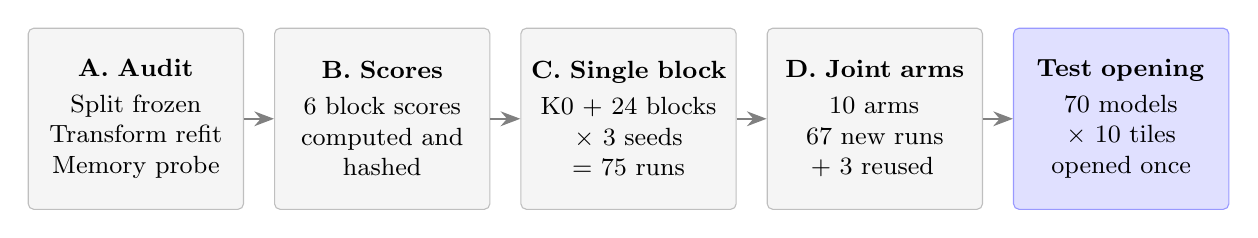
\begin{tikzpicture}[
  stage/.style={draw=black!25, fill=black!4, rounded corners=2pt, minimum width=2.7cm, minimum height=2.3cm, align=center, font=\small, text width=2.5cm},
  last/.style={stage, fill=blue!12, draw=blue!40},
  arr/.style={-{Stealth[length=2.5mm]}, thick, gray}]
\node[stage] (a) {\textbf{A. Audit}\\[2pt] Split frozen\\ Transform refit\\ Memory probe};
\node[stage, right=0.38cm of a] (b) {\textbf{B. Scores}\\[2pt] 6 block scores\\ computed and\\ hashed};
\node[stage, right=0.38cm of b] (c) {\textbf{C. Single block}\\[2pt] K0 + 24 blocks\\ $\times$ 3 seeds\\ = 75 runs};
\node[stage, right=0.38cm of c] (d) {\textbf{D. Joint arms}\\[2pt] 10 arms\\ 67 new runs\\ + 3 reused};
\node[last, right=0.38cm of d] (t) {\textbf{Test opening}\\[2pt] 70 models\\ $\times$ 10 tiles\\ opened once};
\draw[arr] (a) -- (b); \draw[arr] (b) -- (c); \draw[arr] (c) -- (d); \draw[arr] (d) -- (t);
\end{tikzpicture}
\caption{The five Phase 3 stages. Each stage was approved and frozen (scores, thresholds, arms or analysis code hashed) before it ran, and its outcome selected the next stage's design only through rules written in advance.}
\label{fig:stages}
\end{figure*}

\section{Block Scores (Stage B)}
\label{sec:scores}

Every score gives one number per block $\ell = 0, \dots, 23$ and was computed and hashed before any LoRA run in Stage C.

\subsection{Label-free signals}

\textbf{DSS-R2.} The Phase 2 definition (cosine distance of target features from the source centroid, standardised by a source-only baseline), with the roles reversed. The source centroid uses 16 Vaihingen training tiles, the source-only baseline uses matched draws from the 20 Vaihingen training tiles, and the target features come from the 5 Potsdam probe tiles.

\textbf{GSD-perturbation sensitivity.} This new score simulates the change in ground sampling distance on source images only. To make a 9\,cm Vaihingen crop look like a 5\,cm Potsdam crop, we take a window of $n = \text{round}(224 \cdot 5/9) = 124$ pixels, which covers the same ground as a 224-pixel Potsdam crop, and upsample it bilinearly to $224 \times 224$. The score is the relative change of the pooled block feature $f_\ell$:
\begin{equation}
    s_\ell = \frac{1}{N}\sum_{x,c} \frac{\lVert f_\ell(g(x)_c) - f_\ell(x_c) \rVert_2}{\lVert f_\ell(x_c) \rVert_2}
\end{equation}
over source images $x$ and the 9 fixed crop centres $c$.

\textbf{Input-output similarity.} $1 - \overline{\cos}(h_\ell^{\text{in}}, h_\ell^{\text{out}})$ over probe-image tokens, which is high when a block changes its input a lot.

\textbf{Activation norm.} The mean $\lVert h_\ell^{\text{out}} \rVert_2$ over probe-image tokens.

\subsection{Label-using references}

\textbf{Fisher.} Using the frozen backbone, the final decoder of the same-seed decoder-only run and LoRA in all 24 blocks ($B = 0$), we average $\lVert \partial \mathcal{L} / \partial B_{q,\ell} \rVert^2 + \lVert \partial \mathcal{L} / \partial B_{v,\ell} \rVert^2$ over 64 training batches of 8 crops, and then over the three seeds.

\textbf{LogME.} For each block we take the frozen patch tokens of 2,000 random training crops, label each $16 \times 16$ patch by its majority class (purity at least 0.8, at most 4,000 patches per class), and compute the LogME evidence \cite{you2021logme}.

\subsection{Frozen depth prior}

Phase 2 showed an upside-down U shape of utility over depth. We turned it into a fixed prior by fitting a quadratic to the Phase 2 mean utility:
\begin{equation}
\begin{split}
    p(\ell) = {} & -1.8386 \times 10^{-4}\,\ell^2 \\
    & + 4.9992 \times 10^{-3}\,\ell - 4.1343 \times 10^{-4}
\end{split}
\end{equation}
This prior was never refitted. Its top three blocks are L14, L13 and L15, which form the Prior-3 arm.

\section{Screening Gate (Stage C)}

For each block we measure the mean utility $\bar U_\ell$ over three seeds, as in Phase 2. A label-free score $s$ passes the screening gate only if it adds information beyond the depth prior. We compute the residual rank correlation
\begin{equation}
    r_{\text{res}} = \rho_{\text{Spearman}}\bigl(s,\; z(\bar U) - z(p)\bigr)
\end{equation}
where $z$ standardises across the 24 blocks. A score passes if all four conditions hold: $r_{\text{res}} \geq 0.30$; every leave-one-seed-out $r_{\text{res}} \geq 0.15$; the 2.5th percentile of a tile bootstrap (8 validation tiles, 10,000 resamples) is at least 0; and its top-3 regret is no worse than the prior's. At most one passing score could enter Stage D. Under the Phase 2 noise model, an uninformative score passes about 7 to 8\% of the time, so the gate is a screen and not a statistical test.

\section{Stage D Arms and Budget Matching}

LoRA of rank $r$ on the query and value projections of one block adds $2 \times r \times (1024 + 1024) = 4{,}096\,r$ parameters. So three blocks at rank 8 and all 24 blocks at rank 1 both use exactly
\begin{equation}
    3 \times 32{,}768 = 24 \times 4{,}096 = 98{,}304
\end{equation}
LoRA parameters. Uniform rank 1 uses $\alpha = 2$, keeping $\alpha/r = 2$ as in every rank-8 run. The protocol fixed three scenarios in advance, chosen by the Stage C outcome. Since no label-free score passed but the depth prior still correlated with Potsdam utility at $\rho \geq 0.3$, scenario S2 applied, with the arms in Table~\ref{tab:arms}.

\begin{table}[t]
\centering
\caption{Stage D arms (scenario S2). K = 3 arms use rank 8 and match uniform rank 1 in LoRA parameters (98,304). Random-3 uses 10 fixed draws, one seed each.}
\label{tab:arms}
\small
\setlength{\tabcolsep}{4pt}
\begin{tabular}{@{}llc@{}}
\toprule
\textbf{Arm} & \textbf{Blocks} & \textbf{Seeds} \\
\midrule
K0 (decoder only) & none & 10 \\
Prior-3 & L13, L14, L15 & 10 \\
Uniform rank 1 & all 24, $r = 1$ & 10 \\
Middle-3 & L10, L11, L12 & 5 \\
Late-3 & L21, L22, L23 & 5 \\
DSS-R2-3 & L3, L4, L5 & 5 \\
Fisher-3 & L12, L18, L21 & 5 \\
LogME-3 & L6, L7, L8 & 5 \\
Random-3 & 10 draws & 10 \\
Uniform rank 8 & all 24, $r = 8$ & 5 \\
\bottomrule
\end{tabular}
\end{table}

\section{Confirmatory Test (C3)}

Scenario S2 has a single confirmatory contrast, fixed before Stage D:
\begin{quote}
\textit{C3: Prior-3 is non-inferior to uniform rank 1 on the Potsdam test set, with a margin of $\delta = 0.010$ mIoU.}
\end{quote}
For each of the 10 seeds we compute $d_s = \text{mIoU}_{\text{Prior-3}}(s) - \text{mIoU}_{\text{Uniform-r1}}(s)$ on the test set. C3 holds if the lower bound of the 95\% $t$-interval of the mean difference (9 degrees of freedom) is above $-\delta$. As a robustness check we also resample the 10 test tiles 10,000 times (seed 20261111). All other arm comparisons are descriptive. The analysis script was hashed into the test manifest before the first test tile was opened.

% =======================================================
% ============ CHAPTER 4: EXPERIMENTAL SETUP ============
% =======================================================
\chapter{Experimental Setup}
\label{ch:setup}

\section{Datasets and Roles}

We use the same ISPRS IRRG orthophotos as in Phase 2 \cite{rottensteiner2012isprs}, with six classes: impervious surfaces, building, low vegetation, tree, car and clutter. The roles are reversed (Table~\ref{tab:datasets}). Figure~\ref{fig:datasets} shows one crop from each city.

\begin{figure}[t]
\centering
\begin{subfigure}[b]{0.48\columnwidth}
\centering
\includegraphics[width=\linewidth]{vaihingen_area12.png}
\caption{Vaihingen, source (9 cm)}
\end{subfigure}\hfill
\begin{subfigure}[b]{0.48\columnwidth}
\centering
\includegraphics[width=\linewidth]{potsdam_top_3_13.png}
\caption{Potsdam, target (5 cm)}
\end{subfigure}
\caption{IRRG crops of the two cities, each covering 50 m $\times$ 50 m and shown at the same size. In Phase 3 Vaihingen is the source and Potsdam the target. Imagery: ISPRS 2D Semantic Labeling benchmark.}
\label{fig:datasets}
\end{figure}

\begin{table}[t]
\centering
\caption{Dataset roles in Phase 3.}
\label{tab:datasets}
\small
\begin{tabular}{@{}lcc@{}}
\toprule
\textbf{Property} & \textbf{Vaihingen} & \textbf{Potsdam} \\
\midrule
Role & Source & Target \\
Resolution & 9 cm & 5 cm \\
Tile size & smaller, varies & 6,000 px \\
Tiles used & 20 (train) & 38 \\
Labels used & No & Yes \\
\bottomrule
\end{tabular}
\end{table}

Only the images of the 20 Vaihingen training tiles from the Phase 2 split are used. They refit the fixed radiometric transform and form the source pool for the label-free scores. The Vaihingen validation and locked test tiles are not used.

\section{Potsdam Split}

Before any Potsdam label was read, we sorted the 38 tile names and assigned them by position, with no shuffling (Table~\ref{tab:split}). The split file was hashed, and a guard in the data loader refused any label or image that the current stage was not allowed to open.

\begin{table}[t]
\centering
\caption{The frozen Potsdam split. The 5 probe tiles are part of the 20 training tiles.}
\label{tab:split}
\small
\begin{tabular}{@{}lcl@{}}
\toprule
\textbf{Group} & \textbf{Tiles} & \textbf{Used for} \\
\midrule
Train only & 15 & Training, Fisher, LogME \\
Train + probe & 5 & Training, label-free scores \\
Validation & 8 & mIoU, utility \\
Test & 10 & One final opening \\
\midrule
Total & 38 & \\
\bottomrule
\end{tabular}
\end{table}

\section{Training Settings}

All runs use the frozen Phase 2 recipe: Prithvi-EO-2.0-300M, LoRA on Q and V with $\alpha / r = 2$, the decoder on block L23, cross-entropy plus Dice loss, AdamW with learning rate $10^{-3}$ and weight decay 0.01, warm-up and cosine schedule, 2,000 steps, batches of 8 crops of $224 \times 224$, flips and $90^\circ$ rotations, and FP32. Evaluation uses the final step-2,000 checkpoint only. Table~\ref{tab:params} gives the trainable parameters.

\begin{table}[t]
\centering
\caption{Trainable parameters. The 303.9M backbone weights are frozen.}
\label{tab:params}
\small
\setlength{\tabcolsep}{4pt}
\begin{tabular}{@{}lrr@{}}
\toprule
\textbf{Arm} & \textbf{LoRA} & \textbf{Total} \\
\midrule
K0 & 0 & 2,766,726 \\
K = 1 (Stage C) & 32,768 & 2,799,494 \\
K = 3, rank 8 & 98,304 & 2,865,030 \\
Uniform rank 1 & 98,304 & 2,865,030 \\
Uniform rank 8 & 786,432 & 3,553,158 \\
\bottomrule
\end{tabular}
\end{table}

\textbf{Seeds.} Seeds are $1000j$ for $j = 1, \dots, 10$. The LoRA $A$ matrix uses a separate generator seeded with the training seed plus 7,000,000. For one seed, every arm starts from the same decoder weights and sees the same crops in the same order, so arm differences are paired by seed. Seeds 1000 to 3000 reproduce the Phase 2D initial states exactly, which we checked by hash before Stage D.

\section{Evaluation}

A Potsdam tile has $6000 \times 6000$ pixels (36 MP). Our Stage A measurements showed that evaluating several such tiles in one process kept growing in memory, so every tile is evaluated in a fresh process that loads the step-2,000 checkpoint, runs a sliding window of $224 \times 224$ with stride 112, and writes that tile's confusion matrix. The pooled mIoU of a model is computed from the summed matrices of its tiles. Training processes never evaluate Potsdam tiles.

\section{Hardware and Safeguards}

All runs used an Apple M5 laptop with 16 GB of shared memory, PyTorch on the MPS backend and Python 3.12. Each process was watched for memory (stop at 10.5 GB, abort at 11.0 GB, hard limit 11.5 GB), swap growth, memory pressure, temperature, sleep, battery level, stalls (no optimizer step for 300 s) and running time. A run stopped by a guard was kept unchanged, recorded in a new version of the run manifest with file hashes, and repeated under a new ID with the same seed and data, only after approval. Nothing was retried automatically.

% =======================================================
% ============ CHAPTER 5: RESULTS & ANALYSIS ============
% =======================================================
\chapter{Results and Analysis}
\label{ch:results}

\section{Stage A: Audit}

The Potsdam image and label archives matched their checksums, and all 38 label files were present. The split was frozen with 20, 8 and 10 tiles. The radiometric transform was refitted on the 20 Vaihingen training images. A colour check stopped the first Stage A attempt because a few pixels of label tile 4\_12 did not match the six class colours exactly. We approved a fixed rule that snaps a pixel to the nearest class colour only when the match is unambiguous, and recorded every snapped tile. The same rule was later needed for test tile 6\_7, where 0.7\% of pixels were snapped with a maximum colour distance of 3, against at least 249 to any other class.

\section{Stage C: Single-Block Utility on Potsdam}

All 75 Stage C runs passed the integrity checks: correct block and seed, unchanged backbone, matching initial states and data stream, exact checkpoint reload, and mIoU recomputed from the saved confusion matrices. The decoder-only validation mIoU was 0.5729, 0.5698 and 0.5646 for the three seeds (mean 0.569). Training took 24.3 hours in total, and the highest process peak was 10.31 GB. Figure~\ref{fig:utilityc} shows the mean utility of each block.

\begin{figure*}[t]
\centering
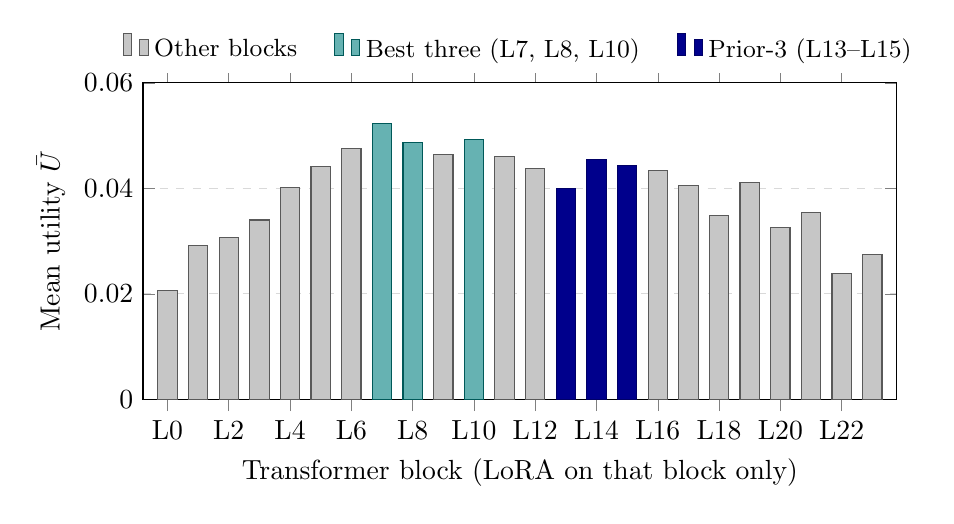
\begin{tikzpicture}
\begin{axis}[
    width=0.92\textwidth, height=5.6cm,
    ybar, bar width=7pt,
    xlabel={Transformer block (LoRA on that block only)}, ylabel={Mean utility $\bar U$},
    xtick={0,2,4,6,8,10,12,14,16,18,20,22},
    xticklabels={L0,L2,L4,L6,L8,L10,L12,L14,L16,L18,L20,L22},
    xmin=-0.8, xmax=23.8, ymin=0, ymax=0.06,
    yticklabel style={/pgf/number format/fixed, /pgf/number format/precision=3},
    scaled y ticks=false,
    ymajorgrids=true, grid style={dashed, gray!30},
    bar shift=0pt,
    legend style={at={(0.5,1.03)}, anchor=south, font=\small, draw=none, legend columns=3, /tikz/every even column/.append style={column sep=0.4cm}},
]
\addplot[fill=gray!45, draw=gray!70!black] coordinates {
(0,0.0206) (1,0.0292) (2,0.0306) (3,0.0340) (4,0.0402) (5,0.0442) (6,0.0476) (9,0.0464) (11,0.0460) (12,0.0438)
(16,0.0434) (17,0.0405) (18,0.0349) (19,0.0411) (20,0.0326) (21,0.0355) (22,0.0238) (23,0.0275)};
\addplot[fill=teal!60, draw=teal!70!black] coordinates {(7,0.0523) (8,0.0487) (10,0.0493)};
\addplot[fill=blue!55!black, draw=blue!40!black] coordinates {(13,0.0400) (14,0.0455) (15,0.0444)};
\legend{Other blocks, Best three (L7{,} L8{,} L10), Prior-3 (L13--L15)}
\end{axis}
\end{tikzpicture}
\caption{Mean utility of each block on Potsdam validation over 3 seeds, measured against the same-seed decoder-only run (mean 0.569). All 24 blocks help. The best block is L7 (+0.052) and the best three are L7, L10 and L8. The frozen depth prior's blocks (L13 to L15) are good but not the best.}
\label{fig:utilityc}
\end{figure*}

Three points stand out. First, every block helps, from +0.021 at L0 to +0.052 at L7, while in Phase 2 block L0 slightly hurt. Second, the curve still rises and then falls, but the peak moved earlier, from L16 in Phase 2 to L7 here. Third, the frozen depth prior still correlates with Potsdam utility ($\rho = 0.533$, Kendall 0.370), above the 0.3 threshold set in advance, so the prior counts as transferred. The Late rule, which prefers the deepest blocks, does not ($\rho = -0.125$). The mean seed standard deviation per block was 0.0043.

\section{Stage C: Screening the Block Scores}

Table~\ref{tab:gate} shows each score against the measured utility and the four gate conditions.

\begin{table*}[t]
\centering
\caption{Stage C screening. $\rho$ is the Spearman correlation with $\bar U$, $r_{\text{res}}$ the residual correlation after the depth prior, LOSO the smallest leave-one-seed-out $r_{\text{res}}$, Boot the tile-bootstrap 2.5th percentile, and Regret the top-3 regret (the prior's is 0.0205). Fisher and LogME use labels and are references only.}
\label{tab:gate}
\small
\begin{tabular}{@{}llcccccc@{}}
\toprule
\textbf{Score} & \textbf{Top 3} & \textbf{$\rho$} & \textbf{$r_{\text{res}}$} & \textbf{LOSO} & \textbf{Boot} & \textbf{Regret} & \textbf{Gate} \\
\midrule
DSS-R2 & L4, L5, L3 & 0.476 & 0.446 & 0.367 & 0.384 & 0.0319 & fail (regret) \\
GSD sensitivity & L14, L13, L12 & 0.528 & $-0.057$ & $-0.078$ & $-0.106$ & 0.0210 & fail \\
IO-similarity & L0, L1, L2 & $-0.204$ & 0.583 & 0.570 & 0.554 & 0.0699 & fail (regret) \\
Activation norm & L23, L0, L22 & $-0.709$ & $-0.052$ & $-0.050$ & $-0.116$ & 0.0784 & fail \\
\midrule
Fisher (labels) & L12, L18, L21 & $-0.126$ & $-0.747$ & $-0.758$ & $-0.767$ & 0.0361 & reference \\
LogME (labels) & L7, L6, L8 & 0.496 & 0.336 & 0.260 & 0.220 & 0.0017 & reference \\
\midrule
Depth prior & L14, L13, L15 & 0.533 & -- & -- & -- & 0.0205 & transfers \\
\bottomrule
\end{tabular}
\end{table*}

No label-free score passed. DSS-R2 and input-output similarity carried information beyond the prior ($r_{\text{res}}$ of 0.446 and 0.583, stable across seeds and tiles), but their top three blocks were worse than the prior's, so they failed the regret condition. GSD sensitivity mostly copied the depth prior (its top three are almost the prior's), and activation norm was negatively related to utility. Among the label-using references, LogME found almost the best blocks (regret 0.0017), while Fisher's ranking was opposite to the residual utility.

DSS-R2 deserves a note. In Phase 2 its top blocks were the deepest ones, while on Potsdam its top blocks are L3 to L5, near the start of the network. A score that points to opposite ends of the network depending on the direction of transfer is not a stable guide for choosing blocks. By the rules written in advance, scenario S2 applied and C3 became the single confirmatory contrast.

\section{Stage D: Joint Adaptation}

All 67 Stage D runs finished 2,000 steps and passed the same integrity checks as Stage C. Training took 24.1 hours in total and the highest process peak was 10.35 GB (uniform rank 1, seed 4000), under the 10.5 GB stop rule. Three runs were stopped by guards (the laptop sleeping on battery, swap growth while other apps were open, and a slow period over the runtime limit) and repeated under new IDs with the same seed and data. Table~\ref{tab:stagedval} gives the validation results.

\begin{table}[t]
\centering
\caption{Stage D validation mIoU (Potsdam, 8 tiles, step 2,000). Gain is over the K0 mean (0.5694).}
\label{tab:stagedval}
\small
\setlength{\tabcolsep}{4pt}
\begin{tabular}{@{}lccc@{}}
\toprule
\textbf{Arm} & \textbf{$n$} & \textbf{mIoU} & \textbf{Gain} \\
\midrule
Uniform rank 8 & 5 & 0.6810 & +0.112 \\
\textbf{Uniform rank 1} & 10 & \textbf{0.6647} & \textbf{+0.095} \\
Random-3 & 10 & 0.6392 & +0.070 \\
Fisher-3 & 5 & 0.6335 & +0.064 \\
LogME-3 & 5 & 0.6322 & +0.063 \\
Middle-3 & 5 & 0.6297 & +0.060 \\
Prior-3 & 10 & 0.6292 & +0.060 \\
DSS-R2-3 & 5 & 0.6267 & +0.057 \\
Late-3 & 5 & 0.6169 & +0.048 \\
K0 & 10 & 0.5694 & 0 \\
\bottomrule
\end{tabular}
\end{table}

At the matched budget, uniform rank 1 was clearly ahead of every 3-block arm. On validation, Prior-3 minus uniform rank 1 was $-0.0355$ on average with a standard deviation of only 0.0019, negative on all 10 seeds. The best 3-block arm was Random-3, ahead of every score-chosen set.

\section{Potsdam Test Opening}

After all 70 models (67 Stage D models and the 3 reused Stage C baselines) were integrity-checked, we froze a test manifest with every checkpoint hash, the 10 test tiles, and the hashes of the code and the analysis script. Each of the 700 tile evaluations ran in its own process, which could open only its own test tile. Every result file confirmed that only that tile's image and label were opened. One evaluation was stopped when a tile passed the 400-second per-tile limit during a temporary slowdown of the GPU (memory was normal). With approval, the run was resumed with a 900-second limit set in a separate launcher, so the hashed code was unchanged. The 97 finished tiles were kept, and the stopped tile was evaluated again from the start. Tile evaluations took about 130 to 145 seconds each, and the highest process peak was 6.0 GB.

\subsection{Confirmatory result}

Table~\ref{tab:c3} and Figure~\ref{fig:c3} give the C3 result.

\begin{table}[t]
\centering
\caption{Contrast C3 on the Potsdam test set (10 seeds, paired).}
\label{tab:c3}
\small
\begin{tabular}{@{}ll@{}}
\toprule
\textbf{Quantity} & \textbf{Value} \\
\midrule
Mean difference & $-0.0341$ \\
Standard deviation & 0.0070 \\
95\% $t$-interval & $[-0.0392,\ -0.0291]$ \\
Required lower bound & $> -0.010$ \\
Seeds with Prior-3 worse & 10 of 10 \\
Tile bootstrap 95\% & $[-0.0387,\ -0.0304]$ \\
Resamples above $-0.010$ & 0\% \\
\midrule
C3 (non-inferiority) & \textbf{not supported} \\
\bottomrule
\end{tabular}
\end{table}

\begin{figure}[t]
\centering
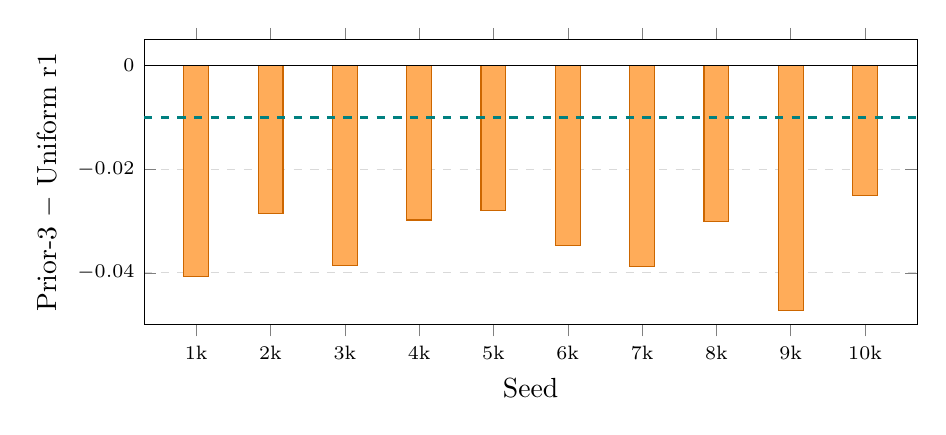
\begin{tikzpicture}
\begin{axis}[
    width=0.94\columnwidth, height=5.2cm,
    ybar, bar width=9pt,
    xlabel={Seed}, ylabel={Prior-3 $-$ Uniform r1},
    xtick={1,...,10}, xticklabels={1k,2k,3k,4k,5k,6k,7k,8k,9k,10k},
    x tick label style={font=\scriptsize},
    xmin=0.3, xmax=10.7, ymin=-0.05, ymax=0.005,
    yticklabel style={/pgf/number format/fixed, /pgf/number format/precision=2, font=\scriptsize},
    scaled y ticks=false,
    ymajorgrids=true, grid style={dashed, gray!30},
]
\addplot[fill=orange!65, draw=orange!80!black] coordinates {
(1,-0.0407) (2,-0.0285) (3,-0.0386) (4,-0.0298) (5,-0.0280) (6,-0.0348) (7,-0.0387) (8,-0.0300) (9,-0.0473) (10,-0.0250)};
\draw[teal, thick, dashed] (axis cs:0.3,-0.01) -- (axis cs:10.7,-0.01);
\draw[black] (axis cs:0.3,0) -- (axis cs:10.7,0);
\end{axis}
\end{tikzpicture}
\caption{Test-set difference between Prior-3 and uniform rank 1 for each seed. The dashed line is the non-inferiority margin ($-0.010$). Every seed is far below it.}
\label{fig:c3}
\end{figure}

The lower bound of the interval is about 0.029 below the margin, so non-inferiority is clearly rejected. The result does not depend on the choice of interval: the tile bootstrap gives almost the same range, and none of its 10,000 resamples came within the margin. The one-sided $p$-value for non-inferiority is essentially 1.

\subsection{All arms on the test set}

Table~\ref{tab:test} reports every arm on the test set. These numbers are descriptive.

\begin{table*}[t]
\centering
\caption{Potsdam test results (10 tiles) for all 70 models. mIoU is the mean over seeds with its 95\% interval, Gain is over the K0 mean (0.5285), and the class columns are mean IoU. Val is the validation mean from Table~\ref{tab:stagedval}.}
\label{tab:test}
\small
\setlength{\tabcolsep}{3pt}
\begin{tabular}{@{}lcccccccccc@{}}
\toprule
\textbf{Arm} & \textbf{$n$} & \textbf{Test mIoU} & \textbf{95\% interval} & \textbf{Gain} & \textbf{Val} & \textbf{Imp.} & \textbf{Bldg.} & \textbf{Low veg.} & \textbf{Tree} & \textbf{Car} \\
\midrule
Uniform rank 8 & 5 & 0.6270 & [0.6239, 0.6301] & +0.0985 & 0.6810 & 0.735 & 0.760 & 0.630 & 0.667 & 0.742 \\
\textbf{Uniform rank 1} & 10 & \textbf{0.6155} & [0.6106, 0.6203] & \textbf{+0.0869} & 0.6647 & 0.712 & 0.755 & 0.622 & 0.659 & 0.722 \\
Random-3 & 10 & 0.5904 & [0.5866, 0.5942] & +0.0619 & 0.6392 & 0.687 & 0.727 & 0.607 & 0.638 & 0.704 \\
Fisher-3 & 5 & 0.5835 & [0.5794, 0.5875] & +0.0549 & 0.6335 & 0.684 & 0.728 & 0.600 & 0.629 & 0.698 \\
LogME-3 & 5 & 0.5818 & [0.5769, 0.5866] & +0.0532 & 0.6322 & 0.676 & 0.709 & 0.605 & 0.636 & 0.695 \\
Middle-3 & 5 & 0.5816 & [0.5786, 0.5847] & +0.0531 & 0.6297 & 0.676 & 0.727 & 0.600 & 0.624 & 0.703 \\
Prior-3 & 10 & 0.5813 & [0.5786, 0.5841] & +0.0528 & 0.6292 & 0.681 & 0.708 & 0.601 & 0.623 & 0.699 \\
DSS-R2-3 & 5 & 0.5777 & [0.5714, 0.5840] & +0.0492 & 0.6267 & 0.670 & 0.689 & 0.608 & 0.635 & 0.695 \\
Late-3 & 5 & 0.5704 & [0.5657, 0.5750] & +0.0418 & 0.6169 & 0.664 & 0.710 & 0.593 & 0.611 & 0.673 \\
K0 & 10 & 0.5285 & [0.5245, 0.5325] & 0 & 0.5694 & 0.637 & 0.651 & 0.568 & 0.566 & 0.623 \\
\bottomrule
\end{tabular}
\end{table*}

\begin{figure}[t]
\centering
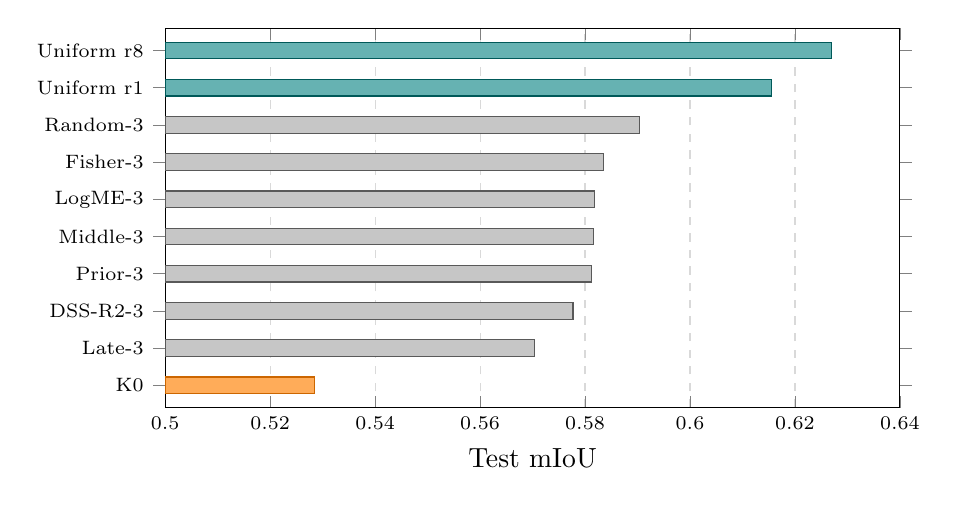
\begin{tikzpicture}
\begin{axis}[
    width=0.9\columnwidth, height=6.4cm,
    xbar, bar width=6pt,
    xlabel={Test mIoU},
    ytick={1,...,10},
    yticklabels={K0, Late-3, DSS-R2-3, Prior-3, Middle-3, LogME-3, Fisher-3, Random-3, Uniform r1, Uniform r8},
    y tick label style={font=\scriptsize},
    x tick label style={font=\scriptsize, /pgf/number format/fixed, /pgf/number format/precision=2},
    xmin=0.5, xmax=0.64, ymin=0.4, ymax=10.6,
    xmajorgrids=true, grid style={dashed, gray!30},
]
\addplot[fill=orange!65, draw=orange!80!black, bar shift=0pt] coordinates {(0.5285,1)};
\addplot[fill=gray!45, draw=gray!70!black, bar shift=0pt] coordinates {(0.5704,2) (0.5777,3) (0.5813,4) (0.5816,5) (0.5818,6) (0.5835,7) (0.5904,8)};
\addplot[fill=teal!60, draw=teal!70!black, bar shift=0pt] coordinates {(0.6155,9) (0.6270,10)};
\end{axis}
\end{tikzpicture}
\caption{Test mIoU of every arm. Uniform LoRA (green) beats every 3-block arm (grey) and the decoder-only baseline (orange).}
\label{fig:testarms}
\end{figure}

Four results stand out (Figure~\ref{fig:testarms}). First, adapting the backbone helps a lot on held-out tiles: every arm gains between +0.042 and +0.099 over the decoder-only baseline, and the intervals across seeds are narrow. Second, uniform rank 1 keeps 88\% of the gain of uniform rank 8 ($0.0869 / 0.0985$) with one eighth of its LoRA parameters. Third, no block-scoring method beat random selection: Random-3 was the best 3-block arm, and paired by seed with uniform rank 1, the 3-block arms were behind by 0.025 (Random-3) to 0.043 (Late-3). Fourth, the arm ranking on the test set is exactly the same as on validation, and every arm loses a similar 0.04 to 0.05 from validation to test, which suggests that the validation tiles were not overfitted. The car class gains the most from adaptation, and clutter (not shown, IoU 0.13 to 0.23) stays the hardest class for every arm.

% =======================================================
% ============ CHAPTER 6: DISCUSSION & LIMITATIONS ======
% =======================================================
\chapter{Discussion and Limitations}
\label{ch:discussion}

\section{What the Results Mean}

The main lesson of Phase 3 is that, for this backbone and this kind of shift, where the LoRA parameters go matters more than which blocks a score picks. Giving every block a very small update was better than giving three blocks a larger one, no matter how those three blocks were chosen. The single-block study explains part of this. Every block gives a real gain on its own, so a method that leaves 21 of 24 blocks untouched gives up gains that a rank-1 update can collect almost for free.

The block scores did not help. The label-free scores either copied the depth prior or pointed to the wrong blocks, and DSS-R2 picked opposite ends of the network in the two transfer directions. Even the label-using LogME score, which found almost the best single blocks, did not make LogME-3 better than Random-3 when the three blocks were trained together. This suggests that adding up single-block gains does not predict how a set of blocks behaves when trained jointly.

\begin{table}[t]
\centering
\caption{Summary of the Phase 3 evidence.}
\label{tab:summary}
\small
\begin{tabular}{@{}p{3.6cm}p{3.6cm}@{}}
\toprule
\textbf{Supported} & \textbf{Not supported} \\
\midrule
LoRA gives large, stable test gains (+0.042 to +0.099) & Prior-3 non-inferior to uniform rank 1 (C3) \\
Uniform rank 1 keeps 88\% of rank-8 gain with 1/8 of the LoRA parameters & Any label-free score passing the gate \\
All 24 single blocks help on Potsdam & Score-chosen blocks beating random blocks \\
Same ranking on validation and test & DSS as a stable block selector \\
\bottomrule
\end{tabular}
\end{table}

\section{Why We Trust the Result}

Table~\ref{tab:summary} summarises the evidence. We trust it for five reasons. Every threshold, score, arm and analysis was frozen and hashed before the data that would judge it existed. The confirmatory test was a single pre-registered contrast, so there is no multiple-testing problem. All comparisons are paired by seed with identical starting weights and data order, checked by hash. The effect is large compared with the noise: the C3 difference is about five standard deviations of the paired difference, and it has the same sign on every seed and almost every tile resample. Finally, the test set was opened once, for frozen models, with a hashed analysis script, and every tile result records which files were opened.

\section{Limitations}

All results come from one backbone (Prithvi-EO-2.0-300M) and one pair of datasets (ISPRS Potsdam and Vaihingen), with LoRA on Q and V only, a decoder that reads only block L23 and 2,000 training steps. A different backbone, decoder, training length or kind of shift may change the picture.

Uniform LoRA was tested only at ranks 1 and 8, so we do not know the best rank for a given budget. Full fine-tuning could not be run within the 16 GB memory limit, so we cannot compare against it.

Secondary arms used 5 seeds, and Random-3 used one seed per random draw, so their small differences (for example Fisher-3 against LogME-3) are not reliable. Only the C3 contrast is confirmatory.

The test tiles of one city are spatially close to each other, so the 10-tile bootstrap is a check of tile-to-tile variation within Potsdam, not of other cities.

Finally, the protocol requires a separate dataset, LoveDA \cite{wang2021loveda}, before any general claim about block selection. That replication has not been run yet.

% =======================================================
% ============ CHAPTER 7: CONCLUSION ====================
% =======================================================
\chapter{Conclusion and Future Work}
\label{ch:conclusion}

\section{Conclusion}

Phase 3 tested selective LoRA adaptation of Prithvi-EO-2.0 in the reverse ISPRS direction, Vaihingen to Potsdam, under a protocol frozen in advance. Our findings are as follows.

Adapting the backbone is clearly worthwhile. Every single block helps on Potsdam, and on the held-out test tiles every adaptation arm improves on the decoder-only baseline by +0.042 to +0.099 mIoU.

Block selection, as we tested it, is not. No label-free score passed the screening gate. The pre-registered confirmatory test, that a frozen 3-block depth prior is non-inferior to uniform rank-1 LoRA at the same budget, failed clearly: the prior was 0.0341 mIoU worse (95\% interval $-0.0392$ to $-0.0291$) and worse on all 10 seeds. No score-chosen set of three blocks did better than three random blocks.

Spreading the budget works well. Uniform rank-1 LoRA on all 24 blocks reached 0.615 test mIoU, 88\% of the gain of standard rank-8 LoRA with one eighth of the LoRA parameters. In short: \textit{spread, don't select}.

\section{Future Work}

Each next step will again be frozen before it is run and needs approval. First, we will repeat the single-block study and the key arms on LoveDA \cite{wang2021loveda} (Urban and Rural), a new dataset with different classes and a different kind of shift, which the protocol requires before any general claim. Second, we will open the locked Vaihingen test set once for the 75 Phase 2D models, as planned in the protocol, to check the Phase 2 utility curve on held-out tiles. Third, we will run a small rank sweep for uniform LoRA (ranks 1, 2, 4 and 8) to find the best use of a given budget. Finally, we plan to write up the study as a 4-page IEEE paper for IGARSS 2027, with the working title ``Spread, Don't Select: Budget-Matched LoRA Placement for Cross-Domain Segmentation with Prithvi-EO-2.0''.

% =======================================================
% ==================== REFERENCES =======================
% =======================================================
\small
\setstretch{1.0}
\bibliographystyle{plainnat}
\begin{thebibliography}{50}
\setlength{\itemsep}{1pt}

\bibitem[Ben-David et~al.(2010)]{bendavid2010theory}
Ben-David, S., Blitzer, J., Crammer, K., Kulesza, A., Pereira, F., and Vaughan, J.~W. (2010).
A theory of learning from different domains.
\emph{Machine Learning}, 79(1--2):151--175.

\bibitem[Cong et~al.(2022)]{cong2022satmae}
Cong, Y., Khanna, S., Meng, C., Liu, P., Rozi, E., He, Y., Burke, M., Lobell, D.~B., and Ermon, S. (2022).
SatMAE: Pre-training transformers for temporal and multi-spectral satellite imagery.
In \emph{NeurIPS}.

\bibitem[Ganin et~al.(2016)]{ganin2016domain}
Ganin, Y., Ustinova, E., Ajakan, H., Germain, P., Larochelle, H., Laviolette, F., Marchand, M., and Lempitsky, V. (2016).
Domain-adversarial training of neural networks.
\emph{Journal of Machine Learning Research}, 17(59):1--35.

\bibitem[Gretton et~al.(2012)]{gretton2012kernel}
Gretton, A., Borgwardt, K.~M., Rasch, M.~J., Sch{\"o}lkopf, B., and Smola, A. (2012).
A kernel two-sample test.
\emph{Journal of Machine Learning Research}, 13:723--773.

\bibitem[He et~al.(2022)]{he2022masked}
He, K., Chen, X., Xie, S., Li, Y., Doll{\'a}r, P., and Girshick, R. (2022).
Masked autoencoders are scalable vision learners.
In \emph{Proceedings of the IEEE/CVF CVPR}, pages 16000--16009.

\bibitem[Houlsby et~al.(2019)]{houlsby2019parameter}
Houlsby, N., Giurgiu, A., Jastrzebski, S., Morrone, B., de~Laroussilhe, Q., Gesmundo, A., Attariyan, M., and Gelly, S. (2019).
Parameter-efficient transfer learning for NLP.
In \emph{ICML}, pages 2790--2799.

\bibitem[Hu et~al.(2022)]{hu2022lora}
Hu, E.~J., Shen, Y., Wallis, P., Allen-Zhu, Z., Li, Y., Wang, S., Wang, L., and Chen, W. (2022).
LoRA: Low-rank adaptation of large language models.
In \emph{ICLR}.

\bibitem[Jakubik et~al.(2023)]{jakubik2023foundation}
Jakubik, J., Roy, S., Phillips, C.~E., et~al. (2023).
Foundation models for generalist geospatial artificial intelligence.
\emph{arXiv preprint arXiv:2310.18660}.

\bibitem[Kirkpatrick et~al.(2017)]{kirkpatrick2017overcoming}
Kirkpatrick, J., Pascanu, R., Rabinowitz, N., et~al. (2017).
Overcoming catastrophic forgetting in neural networks.
\emph{Proceedings of the National Academy of Sciences}, 114(13):3521--3526.

\bibitem[Kornblith et~al.(2019)]{kornblith2019similarity}
Kornblith, S., Norouzi, M., Lee, H., and Hinton, G. (2019).
Similarity of neural network representations revisited.
In \emph{ICML}, pages 3519--3529.

\bibitem[Lee et~al.(2023)]{lee2023surgical}
Lee, Y., Chen, A.~S., Tajwar, F., Kumar, A., Yao, H., Liang, P., and Finn, C. (2023).
Surgical fine-tuning improves adaptation to distribution shifts.
In \emph{ICLR}.

\bibitem[Raghu et~al.(2017)]{raghu2017svcca}
Raghu, M., Gilmer, J., Yosinski, J., and Sohl-Dickstein, J. (2017).
SVCCA: Singular vector canonical correlation analysis for deep learning dynamics and interpretability.
In \emph{NeurIPS}.

\bibitem[Rottensteiner et~al.(2012)]{rottensteiner2012isprs}
Rottensteiner, F., Sohn, G., Jung, J., Gerke, M., Baillard, C., Benitez, S., and Breitkopf, U. (2012).
The ISPRS benchmark on urban object classification and 3D building reconstruction.
\emph{ISPRS Annals of the Photogrammetry, Remote Sensing and Spatial Information Sciences}, I-3:293--298.

\bibitem[Szwarcman et~al.(2024)]{szwarcman2024prithvi}
Szwarcman, D., Roy, S., Fraccaro, P., et~al. (2024).
Prithvi-EO-2.0: A versatile multi-temporal foundation model for Earth observation applications.
\emph{arXiv preprint arXiv:2412.02732}.

\bibitem[Tuia et~al.(2016)]{tuia2016domain}
Tuia, D., Persello, C., and Bruzzone, L. (2016).
Domain adaptation for the classification of remote sensing data: An overview of recent advances.
\emph{IEEE Geoscience and Remote Sensing Magazine}, 4(2):41--57.

\bibitem[Wang et~al.(2021)]{wang2021loveda}
Wang, J., Zheng, Z., Ma, A., Lu, X., and Zhong, Y. (2021).
LoveDA: A remote sensing land-cover dataset for domain adaptive semantic segmentation.
In \emph{NeurIPS Datasets and Benchmarks Track}.

\bibitem[You et~al.(2021)]{you2021logme}
You, K., Liu, Y., Wang, J., and Long, M. (2021).
LogME: Practical assessment of pre-trained models for transfer learning.
In \emph{ICML}, pages 12133--12143.

\bibitem[Zhang et~al.(2023)]{zhang2023adalora}
Zhang, Q., Chen, M., Bukharin, A., He, P., Cheng, Y., Chen, W., and Zhao, T. (2023).
Adaptive budget allocation for parameter-efficient fine-tuning.
In \emph{ICLR}.

\end{thebibliography}

\end{document}
